\chapter{BIOS}

\section{Odrazový bod}

Aby člověk byl schopen vytvořit emulátor jakéhokoliv systému, je vždy potřeba určitý odrazový bod, od kterého lze
začít implementovat emulátor a který současně slouží i jako test korektnosti jeho fungování. Ve většině případů jde o zaváděcí
program, který inicializuje daný systém. V případě \textit{PlayStationu} se jedná o \textit{Basic Input/Output System (BIOS)},
který je zabudován do \textit{ROM} paměti každé \textit{PlayStation} konzole. Existuje několik verzí \textit{BIOSu}.
Hlavní dělení probíhá podle regionálních/verzních základních desek, kde se rozlišují tři hlavní verze \textit{BIOSu}: \textit{Americký (SCEA)},
\textit{Japonský (SCEI)} a \textit{Evropský (SCEE)}. \textit{Sony} také vytvořilo modifikované verze \textit{BIOSů}, které používalo v konzolích
dalších generací pro hladší emulaci \textit{PlayStation} systému (například systém PlayStation Portable obsahuje upravený \textit{BIOS}, který
přeskakuje bootovací úvodní animaci).

Tento \textit{BIOS} lze využít pro strukturovanou implementaci celého emulátoru, kde je nejprve vytvořena paměťová struktura emulátoru
podle paměťové mapy a poté jsou postupně spouštěny instrukce \textit{BIOSu}. Jakmile emulátor narazí na instrukci, která zahrnuje funkcionalitu
či přístup do ještě neimplementované hardwarové komponenty, emulátor signalizuje chybu a chybějící funkcionalitu je třeba buď plně
implementovat, nebo ji utlumit, v závislosti na její závažnosti a schopnosti systému fungovat bez ní.

\section{Funkce}

Ačkoliv se tomuto zaváděcímu programu v \textit{PlayStation} komunitě říká \textit{BIOS}, 
jedná se v podstatě o velmi odlehčený operační systém, který poskytuje systémová volání pro usnadněný přístup k hardwaru.

Uživatel mohl spustit \textit{PlayStation} konzoli i bez vložené hry do \textit{CD-ROM} 
čtečky a byl uvítán úvodní obrazovkou \textit{BIOSu}, tj. \textit{shellem}. 
V tomto menu měl uživatel možnost spravovat, kopírovat a mazat uložený postup her, pokud byla do konzole připojena speciální paměťová karta a také uživatel mohl
v tomto menu přehrávat \textit{Audio CD}.

Hlavní funkcionalitu \textit{BIOS} však poskytuje prostřednictvím speciálních instrukcí systémových volání nebo speciálních tabulek 
rutin umístěných na začátku paměti \textit{RAM}. Skrze toto \textit{API} \textit{BIOS} nabízí řadu funkcí, jako je například 
přístup k souborovému systému \textit{CD-ROM}, správa paměti, výpis ladění, ale také zpracování výjimek, 
manipulace s řetězci, přístup k \textit{GPU}, \textit{SPU}, \textit{GTE} a mnoho dalších\footnote{PCSX ReARMed HLE BIOS \url{https://github.com/notaz/pcsx_rearmed/blob/master/libpcsxcore/psxbios.c}}.

\section{Fáze BIOSu}

\subsection{Zaváděcí fáze}

Ačkoliv se jednotlivé verze \textit{BIOSu} liší ve své funkcionalitě, všechny následují velmi podobný
zaváděcí proces. Při zapnutí/resetu konzole se \textit{Program Counter} procesoru nastaví na hodnotu
\textbf{0xBFC00000}, což je začátek adresy, kde je uložen \textit{BIOS}. V tomto bodě je uložena resetovací
logika. V prvé řadě jsou registry \textit{CPU} vyčištěny a poté začne inicializovat hardware.

Nejdříve se nastaví registry \textit{paměťového ovladače}. Tento kus hardwaru je diskutabilně do jisté míry zbytkem z reálného
počítače, obsahující informace o velikostech jednotlivých pamětí (\textit{RAM}, \textit{BIOS}, \textit{Scratchpad}, ...).

Dále se odizoluje \textit{vyrovnávací paměť instrukcí}, což způsobí, že všechny zápisy se převedou místo na
sběrnici do této \textit{vyrovnávací paměti}. \textit{BIOS} poté tuto paměť vyplní a vyčistí nulami.

V další fázi \textit{BIOS} přistupuje k \textit{ovladači vyrovnávací paměti} a zapne instrukční a datovou vyrovnávací paměť.
Tato komponenta slouží jako globální vypínač jednotlivých vyrovnávacích pamětí (\textit{d-cache, i-cache, scratchpad}), ovšem podobně
jako \textit{paměťový ovladač}, jde spíše o formalitu, neboť do tohoto ovladače se dále už nepřistupuje.

\textit{BIOS} pak zresetuje \textbf{koprocesor 0} (ovladač výjimek) tak, že všechny jeho registry nastaví na nulu a
utlumí všechny kanály \textit{SPU}.

Pokud \textit{BIOS} běžel na vývojářské verzi konzole, programátor mohl využít \textit{Expansion Port (PIO)}, což
do jisté míry je \textit{GPIO} použitelné pro debugování vývoje hry. Aby \textit{PIO} mohlo být použito,
zařízení na druhé straně muselo zaslat speciální ASCII řetězec: \textit{"Licensed by Sony Computer Entertainment Inc."} kvůli verifikaci.

\subsection{Jádro BIOSu}

Po inicializačním resetu hardware je do paměti zkopírován obraz jádra a spuštěn. 
Jádro zpřístupní svou funkcionalitu tím, že vyplní speciální rutinní tabulky na začátku paměti \textit{RAM}, spustí \textit{shell} a zobrazí úvodní animaci.

\begin{figure}[hbt]
    \centering
    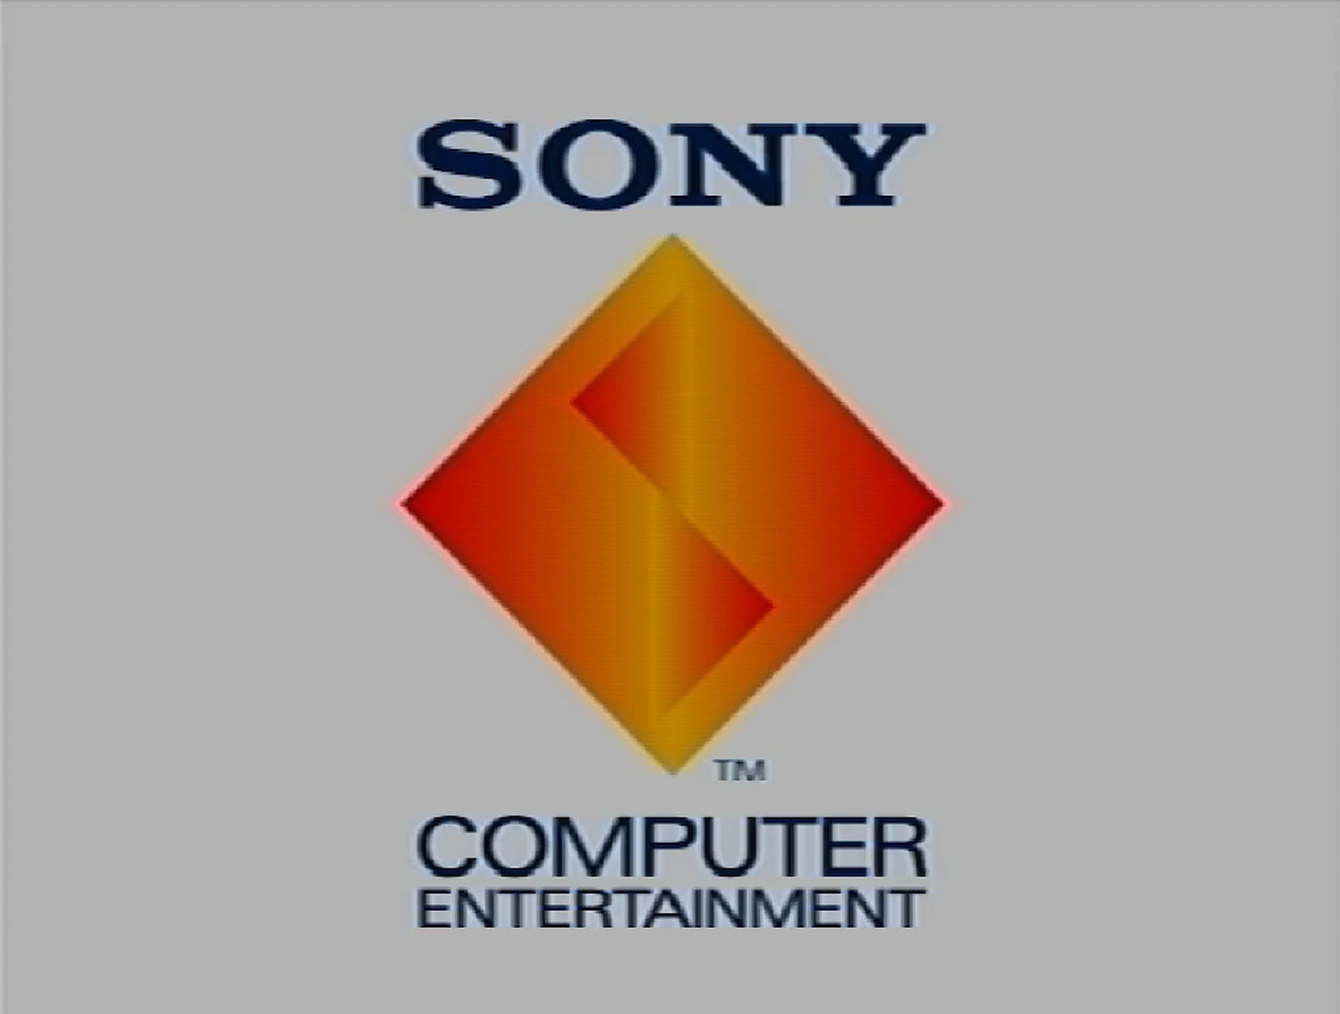
\includegraphics[width=0.8\textwidth]{obrazky-figures/boot-screen.png}
    \caption{Úvodní obrazovka indikující správnou inicializi systému.}
    \label{boot-screen}
\end{figure}

Po dokončení této animace je zkontrolována \textit{CD-ROM} mechanika, zda-li je její poklop uzavřen a zda-li mechanika obsahuje \textit{CD}. 
Pokud jsou tyto podmínky splněny, \textit{BIOS} začne analyzovat souborový systém \textit{CD} a hledat hlavní spustitelný soubor. 
Pokud je přítomen, je posléze spuštěn.

Pokud v \textit{CD-ROM} mechanice nic není, \textit{BIOS} spustí \textit{shell} a dále se již s ničím nadále nezabývá.